\documentclass[tikz,border=10pt]{standalone}
\usepackage{tikz}
\usetikzlibrary{arrows.meta,patterns,decorations.pathmorphing}

\begin{document}
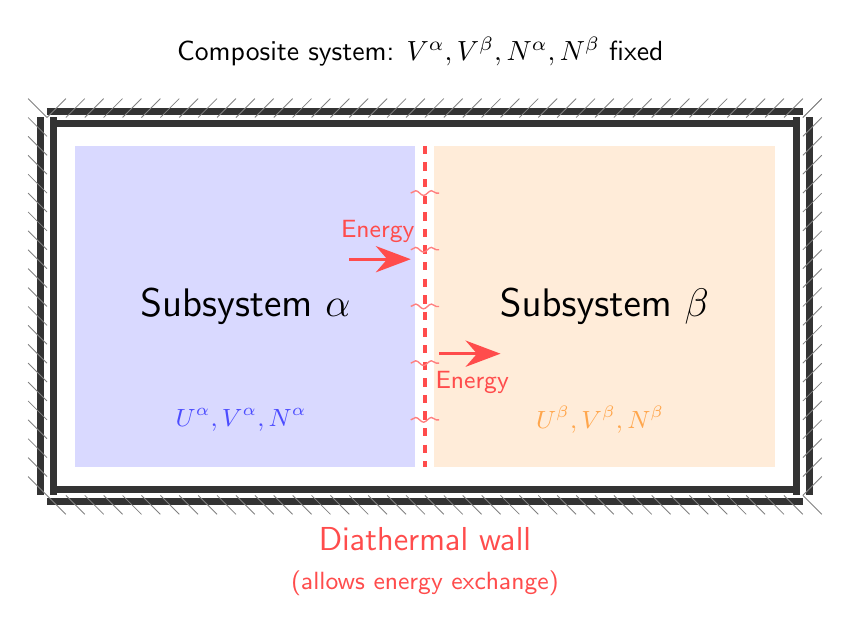
\begin{tikzpicture}[scale=1.2]

    % Define styles
    \tikzset{
        rigid wall/.style={line width=2.5pt, double distance=2pt, draw=black!80},
        diathermal wall/.style={line width=1.5pt, draw=red!70, dashed},
        system box alpha/.style={fill=blue!15, draw=none},
        system box beta/.style={fill=orange!15, draw=none},
        label/.style={font=\Large\sffamily},
        energy arrow/.style={-{Stealth[scale=1.5]}, thick, draw=red!70, line width=1.2pt}
    }

    % Define coordinates for the outer boundary (rigid walls)
    \coordinate (outer-nw) at (-4, 2);
    \coordinate (outer-ne) at (4, 2);
    \coordinate (outer-sw) at (-4, -2);
    \coordinate (outer-se) at (4, -2);

    % Define coordinates for subsystem alpha (left)
    \coordinate (alpha-nw) at (-3.7, 1.7);
    \coordinate (alpha-ne) at (-0.1, 1.7);
    \coordinate (alpha-sw) at (-3.7, -1.7);
    \coordinate (alpha-se) at (-0.1, -1.7);

    % Define coordinates for subsystem beta (right)
    \coordinate (beta-nw) at (0.1, 1.7);
    \coordinate (beta-ne) at (3.7, 1.7);
    \coordinate (beta-sw) at (0.1, -1.7);
    \coordinate (beta-se) at (3.7, -1.7);

    % Draw subsystem alpha (light blue fill)
    \fill[system box alpha] (alpha-sw) rectangle (alpha-ne);

    % Draw subsystem beta (light orange fill)
    \fill[system box beta] (beta-sw) rectangle (beta-ne);

    % Draw the outer rigid walls
    % Top wall
    \draw[rigid wall] (outer-nw) -- (outer-ne);
    % Bottom wall
    \draw[rigid wall] (outer-sw) -- (outer-se);
    % Left wall
    \draw[rigid wall] (outer-nw) -- (outer-sw);
    % Right wall
    \draw[rigid wall] (outer-ne) -- (outer-se);

    % Add diagonal hatching to outer walls
    \foreach \x in {-4,-3.8,...,4} {
        \draw[line width=0.3pt, gray] (\x, 2) -- (\x+0.2, 2.2);
        \draw[line width=0.3pt, gray] (\x, -2) -- (\x+0.2, -2.2);
    }
    \foreach \y in {-2,-1.8,...,2} {
        \draw[line width=0.3pt, gray] (-4, \y) -- (-4.2, \y+0.2);
        \draw[line width=0.3pt, gray] (4, \y) -- (4.2, \y+0.2);
    }

    % Draw the diathermal wall (dashed red line in the middle)
    \draw[diathermal wall] (0, 1.7) -- (0, -1.7);

    % Add wavy lines to indicate energy permeability
    \foreach \y in {-1.2,-0.6,0,0.6,1.2} {
        \draw[red!50, line width=0.5pt, decoration={snake, amplitude=0.3mm, segment length=2mm}, decorate]
            (-0.15, \y) -- (0.15, \y);
    }

    % Energy exchange arrows
    \draw[energy arrow] (-0.8, 0.5) -- (-0.15, 0.5);
    \draw[energy arrow] (0.15, -0.5) -- (0.8, -0.5);

    % Label the subsystems
    \node[label] at (-1.9, 0) {Subsystem $\alpha$};
    \node[label] at (1.9, 0) {Subsystem $\beta$};

    % Label the diathermal wall
    \node[font=\large\sffamily, text=red!70, align=center] at (0, -2.7) {
        Diathermal wall\\
        {\small (allows energy exchange)}
    };

    % Add annotations for subsystems
    \node[font=\small\sffamily, align=center, text=blue!70] at (-1.9, -1.2) {
        $U^\alpha, V^\alpha, N^\alpha$
    };
    \node[font=\small\sffamily, align=center, text=orange!70] at (1.9, -1.2) {
        $U^\beta, V^\beta, N^\beta$
    };

    % Label energy arrows
    \node[font=\small\sffamily, text=red!70] at (-0.5, 0.8) {Energy};
    \node[font=\small\sffamily, text=red!70] at (0.5, -0.8) {Energy};

    % Add constraint annotations
    \node[font=\normalsize\sffamily, align=center] at (0, 2.7) {
        Composite system: $V^\alpha, V^\beta, N^\alpha, N^\beta$ fixed
    };

\end{tikzpicture}
\end{document}
